\documentclass[orivec]{llncs}

\title{A decidable class of (nominal) omega-regular languages over an infinite alphabet}
\author{Vincenzo Ciancia\inst{1} \and Matteo Sammartino\inst{2}}
\institute{ISTI-CNR, Pisa \and Dipartimento di Informatica, Universit\`a di Pisa, Pisa }

\usepackage{amsmath}
\usepackage{amssymb}
\usepackage{tikz}
\usetikzlibrary{arrows,automata,positioning,calc,fit}

\usepackage{cleveref,todonotes,mathpartir}
\usepackage[all]{xy}
\usepackage[utf8]{inputenc}

\SelectTips{cm}{}

\DeclareMathOperator{\dom}{dom}

\newcommand{\todosm}[1]{\todo[size=\tiny]{#1}}

\newcommand{\autom}{\mathcal{A}}
\newcommand{\hdma}{hDMA}
\newcommand{\hdmas}{\hdma s}

% Transition arrows
\newcommand{\Trarrow}{\Longrightarrow}
\newcommand{\Tr}[1]{\overset{#1}{\Trarrow}}
\newcommand{\TrP}[2]{\Tr{#1}_{#2}}
\newcommand{\htrind}[3]{\overset{#1}{\underset{#2}{\trarrow_{#3}}}}
\newcommand{\trind}[2]{\overset{#1}{\trarrow_{#2}}}

\newcommand{\pto}{\rightharpoonup}
\newcommand{\ul}[1]{{\underline{#1}}}
\newcommand{\restr}[2]{\ensuremath{\left.#1\right|_{#2}}}
\newcommand{\lang}{\mathcal{L}}
\newcommand{\syncp}{\otimes}

\newcommand{\tstr}{\mathcal{T}}

\newcommand{\orb}{\mathit{orb}}

\newcommand{\trarrow}{\longrightarrow}
\newcommand{\tr}[1]{\overset{#1}{\trarrow}}

\newcommand{\weight}[1]{|#1|}
\newcommand{\acc}{\mathcal{A}}
\newcommand{\htr}[2]{\overset{#1}{\underset{#2}{\trarrow}}}
\newcommand{\inj}{\rightarrowtail}
\newcommand{\pinj}{\harpoon}
\newcommand{\names}{\mathcal{N}}
\newcommand{\Pow}{\mathcal{P}}

\newcommand{\confs}{\mathcal{C}}
\newcommand{\sub}[2]{[\nicefrac{#1}{#2}]}
%\newcommand{\Im}{\mathit{Im}}

\newcommand{\todocv}[1]{\todo[color=yellow,size=\tiny]{#1}}
\newcommand{\run}{r}
\newcommand{\Inf}{\mathit{Inf}}
\newcommand{\Lang}{\mathcal{L}}
\newcommand{\supp}{\mathit{supp}}
\newcommand{\Perm}{\mathbb{P}}
\renewcommand{\Im}{\mathit{Im}}

\raggedbottom

\begin{document}

\maketitle

\begin{abstract}
 We define a class of languages of infinite words over infinite alphabets, and the corresponding automata. The automata used for recognition are a generalisation of deterministic Muller automata to the setting of nominal sets. Remarkably, the obtained languages are determined by their ultimately periodic fragments, as in the classical case. Closure under complement, union and intersection, and decidability of emptyness and equivalence are preserved by the generalisation. This is shown by using finite representations of the (otherwise infinite-state) defined class of automata.
\end{abstract}

\section{Introduction}\label{sec:introduction}%!TEX root=ndma.tex

% Explain what kind of languages do we get (refer to the example in the paper)

Languages of infinite words are of paramount importance in logics and computer science. Their usage scenarios range from theoretical proofs of decidability for fragments of first-order to applications of relevant practical impact, such as model checking and learning of logical properties. Just as in the classical case, these languages are typically defined on finite alphabets. However, there are cases in which the alphabet is infinite; think e.g., about \emph{data words} \cite{TODO}, or \emph{nominal calculi} \cite{Pi-calculus}. Languages of \emph{finite} words over infinite alphabets have already been studied in the literature, in the form of \emph{register automata} \cite{TODO}. It is nowadays clear that register automata, and languages of infinite alphabets, are also expressible as automata over \emph{nominal sets}, which are in turn equivalent  to history-dependent automata (see \cite{CianciaTuostoTR} for an introduction). 

More recently, the paper \cite{MikLICS} initiated a thorough investigation on the languages that are expressible using variants of nominal sets, and on \emph{nominal computation} in general. The same point of view led to the developments described in \cite{MikPOPL12}, and \cite{PittsPOPL13}. Nominal sets introduce the key notion of \emph{finite support}, that can be roughly explained as a finite memory property with respect to the symbols that appear on a word. From the automata-theoretic perspective, languages of finite words over infinite (nominal) alphabets are treated in a satisfactory way by just defining an automaton as an \emph{orbit-finite} set of states \cite{CiaMonIC}, equipped with an \emph{equivariant} transition relation, and equivariant acceptance condition. Each finite word is finitely supported, thus the set of all words forms a nominal set. 

The case of infinite words over nominal alphabets is more problematic, as an infinite word over an infinite alphabet is generally not finitely supported. Consider a machine that reads any symbol from an infinite, countable alphabet, and never stores it. Clearly, such a machine has finite (empty) memory. The set of its traces is simply described as the set of all infinite words over the alphabet. However, in the language we have various species of words. Some of them are finitely supported; for example, words that consist of the infinite repetition of a finite word. Some others are not finitely supported, such as the word enumerating all the symbols of the alphabet. Such words lay inherently out of the settting of nominal sets. However, the existence of these words does not give to the language infinite memory. More precisely, if we only consider finite-memory machines, problematic words can not be singled out; rather, their presence in a language can not be separated from the presence of an infinite number of other words. The simple machine we described accepts all possible infinite words. A machine that would accept only the enumeration of all symbols, instead, would require infinite memory. 

The aim of this work is to translate the intuitions in the previous paragraphs into precise mathematical terms, in order to define a class of languages of infinite words over infinite alphabets that possess finite-memory properties. We extend the automata over nominal sets of \cite{MikLICS}, also used in \cite{CianciaTuostoTR}, to handle infinite words, by imposing a Muller-automata-alike condition over the \emph{orbits} (not the states!) of the automata. By doing so, it turns out that our languages not only are finite-memory, but they retain computational properties, such as closure under boolean operations and decidability of emptyness (thus, containment and equivalence). Moreover, a somewhat unexpected result is that the obtained languages are determined by their \emph{ultimately periodic} fragments, just as in the classical case. This clarifies why it is not possible to single-out problematic streams, as we explained above. Being determined by ultimately periodic fragments is fundamental for classical automata over infinite words, whose consequences have probably not yet been explored in full. For example, this property makes it possible to learn languages of infinite words \cite{Emerson}, or to find canonical representatives up-to language equivalence, in a coalgebraic flavour \cite{CV12}. 





\section{Background}\label{sec:background}%!TEX root=ndma.tex
\paragraph{Notation.} As a matter of notation, for $X$, $Y$ sets, we let $f \colon X \to Y$ be a total function from $X$ to $Y$, $f \colon X \inj Y$ be a total injective function and $f \colon X \pto Y$ a partial function. We write $\dom(f)$ for the subset of $X$ on which $f$ is defined. For $f$ injective, the expression $f^{-1} \colon Y \pto X$ denotes the the partial inverse function $\{(y,x) \mid f(x) = y \}$. We let $\restr{f}{X'}$, with $X' \subseteq X$, be the domain restriction of $f$ to $X'$. (Partial) function compositions is written $f \circ g$: it maps $x$ to $f(g(x))$ only if $x \in \dom(g)$; $f^n$ is the $n$-fold composition of $f$ with itself. 

We assume an infinite set of names $\names$, and we write $Perm$ for the group of finite-kernel permutations of $\names$, namely those bijections $\pi \colon \names \to \names$ such that the set $\{ a \mid \pi(a) \neq a \}$ is finite.
\begin{definition}
A \emph{nominal set} is a set $X$ along with an action for $Perm$, that is a function $\cdot \colon Perm \times X \to X$ such that, for all $x \in X$ and $\pi,\pi' \in Perm$, $x \cdot id_\names = x$ and $(\pi \circ \pi') \cdot x = \pi \cdot (\pi' \cdot x)$. Also, it is required that each $x \in X$ has \emph{finite support}, meaning that there exists a finite $S \subseteq \names$ such that, $\restr{\pi}{S} = id_S$ implies $\pi \cdot x = x$, for all $\pi \in Perm$.
\end{definition}
%
Given $x \in X$, the \emph{orbit} of $x$, denotedy $\Orb(x) $, is the set $\{ \pi \cdot x \mid \pi \in Perm\} \subseteq X$. We write $\Orb(X)$ for $\{ \Orb(x) \mid x \in X\}$. This set forms a partition of $X$. In particular, $\names$ under the natural permutation action $\pi \cdot a = \pi(a)$, is a nominal set, where each element $a$ is supported by $\{a\}$ and there is just one orbit. 


\section{Nominal regular $\omega$-languages}\label{sec:languages}%!TEX root=ndma.tex

In the following, we extend \emph{Muller automata} to the case of nominal alphabets. Traditionally, automata can be deterministic or non-deterministic. In the case of finite words, non-deterministic nominal automata are not closed under complementation, whereas the deterministic ones are; similar considerations apply to the infinite words case. Thus, we adopt the deterministic setting in order to retain complementation.
%\todo{Questo NON dimostra che i Muller automata non-deterministici nominali non siano chiusi rispetto a complementazione!}
%For each (nominal) automaton on finite words, it is not difficult to find an automaton \todo{not clear} on infinite words which is complementable if and only if the original automaton is. Thus, in order to extend previous results on closure under complementation and decidability, we work with deterministic structures.

\begin{definition}\label{def:ndma}
 A \emph{nominal deterministic Muller automaton} (nDMA) is a tuple $(Q,\tr{},q_0,\acc)$ where:
 
  \begin{itemize}
  \item $Q$ is an orbit-finite nominal set of \emph{states}, with $q_0 \in Q$ the \emph{initial state};
  
  \item $\acc \subseteq \Pow(\orb(Q))$ is a set of sets of orbits, intended to be used as an acceptance condition in the style of Muller automata.
  
  \item $\htr{}{}$ is the \emph{transition relation}, made up of triples $q_1 \tr{a} q_2$, having \emph{source} $q_1$, \emph{target} $q_2$, \emph{label} $a \in \names$;
  
  \item the transition relation is \emph{deterministic}, that is, for each $q \in Q$ and $a \in \names$ there is exactly one transition with source $q$ and label $a$;
  
  \item the transition relation is \emph{equivariant}, that is, invariant under permutation: there is a transition $q_1 \tr a q_2$ if and only if, for all $\pi$, also the transition $\pi \cdot q_1 \tr{\pi(a)} \pi \cdot q_2$ is present.
 \end{itemize}
\end{definition}
%
In nominal sets terminology, the transition relation is an \emph{equivariant function} of type $Q \times \names \to Q$.  Notice that nDMA are infinite state, infinitely branching machines, even if orbit finite. For effective constructions we employ equivalent finite structures (see Section \ref{sec:hd-automata}). Definition \ref{def:ndma} induces a simple definition of acceptance, very close to the classical one. In the following, fix a nDMA $A=(Q,\tr{},q_0,\acc)$.

\begin{definition}
\label{def:inf-word}
 An infinite \emph{word} $\alpha \in \names^\omega$ is an infinite sequence of symbols in $\names$. Words have \emph{point-wise} permutation action, namely $(\pi \cdot \alpha)_i = \pi(\alpha_i)$, making a word finitely supported if and only if it contains finitely many different symbols. 
\end{definition}

\begin{definition}\label{def:nominal-run}
 Given a word $\alpha \in \names^\omega$, a \emph{run} of $\alpha$ from $q \in Q$ is a sequence of states $\run \in Q^\omega$, such that $\run_0 = q$, and for all $i$ we have $\run_i \tr{\alpha_i} \run_{i+1}$. 
 By determinism (see Definition \ref{def:ndma}), for each infinite word $\alpha$, and each state $q$, there is exactly one run of $\alpha$ from $q$, that we call $\run^{\alpha,q}$, or simply $\run^{\alpha}$ when $q=q_0$.
\end{definition}

\begin{definition}\label{def:inf-set}
 For $\run \in Q^\omega$, let $\Inf(\run)$ be the set of \emph{orbits} that $\run$ traverses infinitely often, i.e., $\orb(q) \in \Inf(\run)$ iff. for all $i$, there is $j > i$ s.t. $\run_j \in \orb(q)$.
\end{definition}

\begin{definition}
 A word $\alpha$ is \emph{accepted} by state $q$ whenever $\Inf(\run^{\alpha,q}) \in \acc$. We let $\Lang_{A,q}$ be the set of all accepted words by $q$ in $A$; we omit $A$ when clear from the context, and $q$ when it is $q_0$, thus $\Lang_A$ is the language of the automaton $A$. We say that $\Lang \subseteq \names^\omega$ is a \emph{nominal $\omega$-regular language} if it is accepted by a nDMA.
\end{definition}

\begin{remark}\label{rem:simple-alphabet} We use $\names$ as alphabet. One can chose any orbit-finite nominal set; the definitions of automata and acceptance are unchanged, and finite representations are similar.
%this includes classical finite alphabets, cast as nominal sets under trivial permutation action, the alphabet of \emph{names} $\names$, and more complex structures that can be thought of as \emph{symbols} with attached a list of names and some information about their symmetry (similarly to \cite{MikBartekLICS}). Indeed, the cases where the alphabet is infinite are more interesting; however, 
%
%However, it does not make a great difference, from the mathematical perspective, whether the alphabet has only one orbit having one name (the case of $\names$) or if there are more orbits and names. 
%The definition of automaton and acceptance would be the same, and finite representation would exist.e. 
Using $\names$ simplifies the presentation, especially in Section \ref{sec:hd-automata}.
\end{remark}

\begin{example}\label{exa:session}
 Consider the nDMA in \cref{fig:example-session}. We have $Q = \{q_0\} \cup \{q_a \mid a \in \names\}$. For all $\pi$, we let $\pi \cdot q_0 = q_0$, $\pi \cdot q_a = q_{\pi(a)}$. We have $\supp(q_0) = \emptyset$, and $\supp(q_a) = \{ a \}$. For all $a$, let $q_0 \tr{a} q_a$, $q_a \tr{a} q_0$, and for $b \neq a$, $q_a \tr b q_a$. Each of the infinite ``legs'' of the automaton rooted in $q_0$ remembers a different name, and returns to $q_0$ when the same name is encountered again. There are two orbits, namely $\orb_0 = \{ q_0 \}$ and $\orb_1 = \{ q_a \mid a \in \names \}$. We let $\acc = \{ \{ \orb_0, \orb_1 \} \}$. For acceptance, a word needs to cross both orbits infinitely often. Thus, $\Lang_{q_0}=\{aua \mid a \in \names, u \in (\names\setminus\{a\})^* \}^\omega$.
% 
This is an idealized version of a service, where each in a number of potentially infinite users (represented by names) may access the service, reference other users, and later leave. Infinitely often, an arbitrary symbol occurs, representing an ``access''; the next occurrence of the same symbol denotes a ``leave''. One could use an  alphabet with two infinite orbits to distinguish the two kinds of action (see Remark \ref{rem:simple-alphabet}), or reserve two distinguished names of $\names$ to be used as ``brackets'' 	
%to appear in words 
 before the different occurrences of other names, adding more states.
 %Another option is to add to the alphabet two special symbols without names, say, ``access'' and ``leave'', and additional states and transitions, to appear before the two distinct usages of a symbol.
\end{example}

\begin{figure}[t]
%\begin{center}
\subfigure[]{
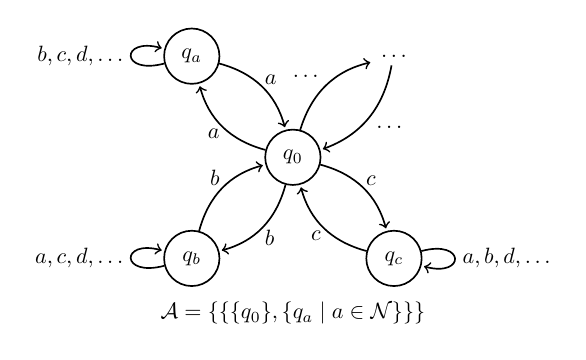
\begin{tikzpicture}[->,shorten >=1pt,auto,node distance=15ex,semithick,initial text={},scale=0.8, every node/.style={scale=0.8}]  
  \node[state] (q0)               {$q_0$};
  \node[state] (qa) [above left of = q0] {$q_a$};
  \node[state] (qb) [below left of = q0] {$q_b$};
  \node[state] (qc) [below right of = q0] {$q_c$};
  \node (qany) [above right of = q0] {$\ldots$};
  	\coordinate (Middle) at ($(qb)!0.5!(qc)$);
  \node (acc) [below=3ex of Middle] {$\acc = \{ \{ \{ q_0 \} , \{ q_a \mid a \in \names \}\}\}$};
% 
%  
  \path (q0) edge [bend left]  node[inner sep=1pt] {$a$} (qa);
  \path (q0) edge [bend left]  node[inner sep=1pt] {$b$} (qb);
  \path (q0) edge [bend left]  node[inner sep=1pt] {$c$} (qc);
  \path (q0) edge [bend left]  node {$\ldots$} (qany);  
  \path (qa) edge [bend left]  node[inner sep=1pt] {$a$} (q0)
             edge [loop left] node {$b,c,d,\ldots$} (qa);  
  \path (qb) edge [bend left]  node[inner sep=1pt] {$b$} (q0)
             edge [loop left] node {$a,c,d,\ldots$} (qb);  
  \path (qc) edge [bend left]  node[inner sep=1pt] {$c$} (q0)
             edge [loop right] node {$a,b,d,\ldots$} (qc);  
  \path (qany) edge [bend left]  node {$\ldots$} (q0);
             edge [loop right] node {} (qany);
%
\end{tikzpicture}
\label{fig:example-session}
}
\hspace{2ex}
\subfigure[]{
{\centering
 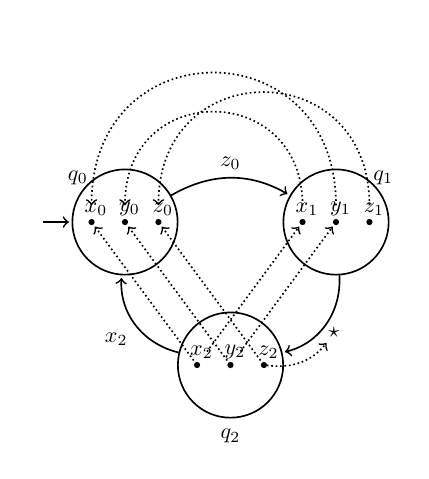
\begin{tikzpicture}[->,shorten >=1pt,auto,node distance=2.8cm,semithick,initial text={},scale=0.8, every node/.style={scale=0.8}] 
\tikzstyle{every state}=[minimum size=10ex]
  \tikzstyle{register}=	[circle,fill,draw,inner sep=0pt,minimum size=2pt]
%	
%
\node[register,label={[shift={(2pt,-2pt)}]above:$x_0$}] (reg00) {};
  \node[register,label={[shift={(2pt,-2pt)}]above:$y_0$}] (reg01) [right=10pt of reg00] {};
  \node[register,label={[shift={(2pt,-2pt)}]above:$z_0$}] (reg02) [right=10pt of reg01] {};
  \node[register,label={[shift={(2pt,-2pt)}]above:$x_1$}] (reg10) [right=50pt of reg02] {};
  \node[register,label={[shift={(2pt,-2pt)}]above:$y_1$}] (reg11) [right=10pt of reg10] {};
  \node[register,label={[shift={(2pt,-2pt)}]above:$z_1$}] (reg12) [right=10pt of reg11] {};
  \node[register,label={[shift={(2pt,-2pt)}]above:$y_2$}] (reg21) at ($(reg02)!0.5!(reg10)$) [yshift=-15ex] {};
  \node[register,label={[shift={(2pt,-2pt)}]above:$x_2$}] (reg20) [left=10pt of reg21] {};
  \node[register,label={[shift={(2pt,-2pt)}]above:$z_2$}] (reg22) [right=10pt of reg21] {};
  \node[state,initial,fit={(reg00) (reg01) (reg02)},inner sep=2ex] (q0) {};
  \node[above left=-1ex of q0] (lab0) {$q_0$}; 
  \node[state,fit={(reg10) (reg11) (reg12)},inner sep=2ex] (q1) {};
  \node[above right=-1ex of q1] (lab1) {$q_1$}; 
  \node[state,fit={(reg20) (reg21) (reg22)},inner sep=2ex] (q2) {};
  \node[below=1pt of q2] (lab2) {$q_2$}; 

  \path (q0) edge [bend left] node {$z_0$} (q1);
  \path (q1) edge [bend left=40]  node[inner sep=1pt] (star) {$\star$} (q2);
  \path (q2) edge [bend left=40] node {$x_2$} (q0);	
  \path (reg10) edge[densely dotted,out=90,in=90,looseness=2,shorten >=5pt,shorten <=5pt] (reg01);
  \path (reg11) edge[densely dotted,out=90,in=90,looseness=2,shorten >=5pt,shorten <=5pt] (reg00);
  \path (reg12) edge[densely dotted,out=90,in=90,looseness=2,shorten >=5pt,shorten <=5pt] (reg02);
  \path (reg20) edge[densely dotted,shorten <=5pt] (reg10);
  \path (reg21) edge[densely dotted,shorten <=5pt] (reg11);
  \path (reg22) edge[bend right,densely dotted] (star);
  \path (reg20) edge[densely dotted,shorten <=1pt] (reg00);
  \path (reg21) edge[densely dotted,shorten <=1pt] (reg01);
  \path (reg22) edge[densely dotted,shorten <=1pt] (reg02);
\end{tikzpicture}
}
\label{fig:upwords-ex}
}
%\end{center}
%
%\vspace{-6.3ex}
%\begin{center}
\subfigure[]{
{
\centering
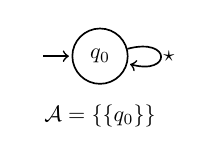
\begin{tikzpicture}[->,shorten >=1pt,auto,node distance=2.8cm,semithick,initial text={},scale=0.8, every node/.style={scale=0.8}]
%
%	
  \node[state,initial] (q0) {$q_0$}; 
  \node[below=1ex of q0] {$\acc = \{ \{ q_0 \} \}$};
%
  \path (q0) edge [loop right]  node[inner sep=1pt] (star) {$\star$} (q0);
\end{tikzpicture}
}
\label{fig:hd-names-omega}
}
%
\hspace{10ex}
\subfigure[]{
{\centering
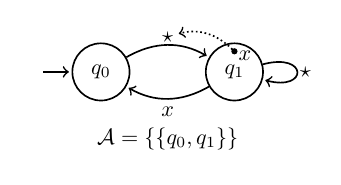
\begin{tikzpicture}[->,shorten >=1pt,node distance=14ex,auto,semithick,initial text={},scale=0.8, every node/.style={scale=0.8}]
  \tikzstyle{every state}=[minimum size=6ex]
  \tikzstyle{register}=	[circle,fill,draw,inner sep=0pt,minimum size=2pt]	
  \node[state,initial] (q0) {$q_0$}; 
  \node[state,right of=q0] (q1) {};  
  \node (lab1) at (q1) {$q_1$};  \node[register,label={[xshift=-3pt,yshift=-2pt]right:$x$}] (reg) [above=1pt of lab1] {};
	\coordinate (Middle) at ($(q0)!0.5!(q1)$);
  \node[below=4ex of Middle] {$\acc = \{\{q_0,q_1\}\}$};
  \path (q0) edge [bend left]  node[inner sep=1pt] (star) {$\star$} (q1);
  \path (q1) edge[loop right] node[inner sep=1pt] {$\star$} (q1);
  \path (q1) edge [bend left] node {$x$} (q0);
  \path (reg) edge[densely dotted,bend right] (star);
\end{tikzpicture}
}
\label{fig:hd-of-example}
}
%\end{center}
\label{fig:automata}
\vskip -10pt
\caption{Some automata, together with their accepting conditions.
%\subref{fig:example-session} is the nDMA of \cref{exa:session} and \subref{fig:hd-of-example} is the corresponding \hdma; \subref{fig:upwords-ex} is an example \hdma\, where we have omitted the accepting condition and irrelevant transitions, all assumed to end up in a sink state without registers; \subref{fig:hd-names-omega} is the \hdma\ recognizing $\names^\omega$.
}\vskip-10pt
\end{figure}

\noindent Accepted words may fail to be finitely supported. However, languages are. This adheres to the intuition that a machine running forever may read an unbounded amount of different pieces of data, but still have finite memory.
%in line with the intuition of studying machines with finite memory, that never halt.

\begin{theorem}\label{thm:languages-finitely-supported}
 For $\Lang$ a language, and $\pi\in \Perm$, let $\pi\cdot \Lang = \{\pi \cdot \alpha \mid \alpha \in \Lang\}$. For each state $q$ of an nDMA, $\Lang_{q}$ is finitely supported.
\end{theorem}

% \todo{
%  Theorems? First of all, finite support of languages. Also: observation that streams are not finitely supported, but languages are. In the example, what are the finitely supported accepted streams (and how do they differ from the infinitely supported ones?). Can we explain in words the ``finite memory determinacy'' of languages?
% }



\section{Finite automata}\label{sec:hd-automata}
%!TEX root=ndma.tex

In this section, we introduce finite representations of nDMAs. These are similar to classical finite-state automata, but each state is equipped with local registers. There is a notion of assignment to registers, and it is possible to accept, and eventually store, \emph{fresh} symbols. Technically, these structures extend \emph{history-dependent automata} (see \cite{Pistore99}), introducing acceptance of infinite words.

\begin{definition}\label{def:hdma}
 An \emph{history-dependent deterministic Muller automaton} (\hdma) is a tuple $(Q,\weight -,q_0,\rho_0,\htr{}{},\acc)$
 where:
 \begin{itemize}
  \item $Q$ is a finite set of \emph{states};
  \item for $q \in Q$, $\weight{q}$ is a finite set of \emph{local names} (or \emph{registers}) of state $q$;
  \item $q_0 \in Q$ is the \emph{initial state};
  \item $\rho_0 : \weight{q_0} \inj \names$ is the \emph{initial assignment};
  \item $\acc \subseteq \Pow(Q)$ is the \emph{accepting condition}, in the style of \emph{Muller automata};
  \item $\htr{}{}$ is the \emph{transition relation}, made up of quadruples $q_1 \htr{l}{\sigma} q_2$, having \emph{source} $q_1$, \emph{target} $q_2$, label $l \in \weight{q_1} \uplus \{\star\}$, and \emph{history} $\sigma : \weight{q_2} \inj \weight{q_1} \uplus \{l\}$;
  \item the transition relation is \emph{deterministic} in the following sense: for each $q_1 \in Q$,   there is exactly one transition with source $q_1$ and label $\star$, and exactly one transition with source $q_1$ and label $x$ for each $x \in \weight{q_1}$.
 \end{itemize}
\end{definition}
%

\begin{remark}
To keep the notation lightweight, we do not use a \emph{symmetry} attached to states of an \hdma. It is well known (see \cite{MontanariP05}) that symmetries are needed for existence of canonical representatives; we consider this aspect out of the scope of this work. Note that (classical) Muller automata do not have canonical representatives up-to language equivalence. To obtain those, one can use two-sorted structures as in \cite{CV12}. Even though this idea could be applied to hDMAs, this is not straightforward, and requires further investigation.
\label{rem:no-symmetry}
\end{remark}
%
In the following we fix a \hdma{} $A = (Q,\weight -,q_0,\rho_0,\htr{}{},\acc)$. We overload notation (e.g., for the inf-set or the unique run of a word) from \cref{sec:languages}, as it will be always clear from the context whether we are referring to an nDMA or to an \hdma. Acceptance of $\alpha \in \names^\omega$ is defined using the \emph{configuration graph} of $A$.

\begin{definition}\label{def:configuration-graph}
 The set $\confs(A)$ of \emph{configurations} of $A$ consists of the pairs $(q,\rho)$ such that $q \in Q$ and $\rho : \weight q \inj \names$ is an injective \emph{assignment} of names to registers.
\end{definition}

\begin{definition}
\label{def:configuration-graph}
The \emph{configuration graph} of $A$ is a graph with edges of the form  
$(q_1,\rho_1) \tr a (q_2,\rho_2)$ where the source and destination are configurations, and $a \in \names$. There is one such edge if and only if there is a transition $q_1 \htr l \sigma q_2$ in $A$ and either of the following happens: 
 \begin{itemize} 
  \item $l \in \weight{q_1}$, $\rho_1(l) = a$, and $\rho_2 = \rho_1 \circ \sigma$;
  \item $l = \star$, $a \notin \Im(\rho_1)$, $\rho_2 = (\rho_1 \circ \sigma)\sub{a}{\sigma^{-1}(\star)}$.
 \end{itemize}
\end{definition}
% 

The definition deserves some explanation. Fix a configuration $(q_1,\rho_1)$. Say that name $a\in \names$ is \emph{assigned to} the register $x \in \weight{q_1}$ if $\rho_1(x) = a$. When $a$ is not assigned to any register, it is \emph{fresh} for a given configuration. Then the transition $q_1 \htr l \sigma q_2$, under the assignment $\rho_1$, consumes a symbol as follows: either $l \in \weight{q_1}$ and $a$ is the name assigned to register $l$, or $l$ is $\star$ and $a$ is fresh. The destination assignment $\rho_2$ is defined using $\sigma$ as a binding between local registers of $q_2$ and local registers of $q_1$, therefore composing $\sigma$ with $\rho_1$ and eventually adding a freshly received name, whenever $\star$ is in the image of $\sigma$. For readability, we assume that the functional update $\sub{a}{\sigma^{-1}(\star)}$ is void when $\star \notin \Im(\sigma)$. The following lemma clarifies the notion of determinism that we use.

\begin{lemma}
\label{lem:deterministic-configuration-graph}
 For each configuration $(q_1,\rho_1)$ and symbol $a \in \names$, there is exactly one configuration $(q_2,\rho_2)$ such that $(q_1,\rho_1) \tr a (q_2,\rho_2)$.
\end{lemma}
%
We use the notation $(q_1,\rho_1) \Tr{v} (q_2,\rho_2)$ to denote a path that spells $v$ in the the configuration graph. Furthermore, we define runs of infinite words.
%

\begin{definition}
 A \emph{run} $\run$ of an infinite word $\alpha \in \names^\omega$ from configuration $(q,\rho)$ is a sequence $(q_i,\rho_i)$ of configurations, indexed by $\omega$, such that $(q_0,\rho_0)=(q,\rho)$ and for all $i$, in the configuration graph, we have $(q_i,\rho_i) \tr{\alpha_i} (q_{i+1},\rho_{i+1})$. 
\end{definition}

\noindent The following is a simple corollary of  \cref{lem:deterministic-configuration-graph}.

\begin{proposition}
\label{prop:unique-path}
Given $(q_1,\rho_1) \in \confs(A)$ and $v \in \names^\omega$, there exists a unique path $(q_1,\rho_1) \Tr{v} (q_2,\rho_2)$ in the configuration graph of $A$. Similarly, for each word $\alpha$ and configuration $(q,\rho)$, there is a unique run $\run^{\alpha,q,\rho}$ from $(q,\rho)$. We omit $q$ and $\rho$ from the notation, when dealing with the \emph{initial configuration} $(q_0,\rho_0)$.
\end{proposition}

\noindent Finally, we define acceptance of \hdmas. 

\begin{definition}\label{def:acceptance-of-hdmas}
 Consider the unique run $\run$ of an infinite word $\alpha$ from configuration $(q,\rho)$. 
 Let $\Inf(\run)$ denote the set  of states that appear infinitely often in the first component of $\run$. By finiteness of $Q$, $\Inf(\run)$ is not empty. The automaton $A$ accepts $\alpha$ whenever $\Inf(r) \in \acc$. In this case, we speak of the \emph{language} $\Lang_A$ of words accepted by the automaton.
\end{definition}
%
%\begin{figure}[t]
%\centering
%\begin{subfigure}[t]{.4\linewidth}
%\centering
% \begin{tikzpicture}[->,>=stealth',shorten >=1pt,auto,node distance=2.8cm,semithick,initial text={}]
%  %\tikzstyle{every state}=[minimum size=10ex]
%  %\tikzstyle{register}=	[circle,fill,draw,inner sep=0pt,minimum size=2pt]
%	
%  \node[state,initial] (q0) {$q_0$}; 
%  \node[right=10ex of q0] {$\acc = \{ \{q_0 \}\}$ };
%
%  \path (q0) edge [loop right]  node[inner sep=1pt] (star) {$\star$} (q0);
%\end{tikzpicture}
%\subcaption{$\autom_\omega$}
%\[ \acc = \{ \{q_0 \}\} \]
%\label{fig:nomega-hdma}
%\end{subfigure}
%
%\begin{subfigure}[t]{.4\linewidth}
%\centering
% \begin{tikzpicture}[->,>=stealth',shorten >=1pt,node distance=14ex,auto,semithick,initial text={}]
%  \tikzstyle{every state}=[minimum size=6ex]
%  \tikzstyle{register}=	[circle,fill,draw,inner sep=0pt,minimum size=2pt]
%	
%  \node[state,initial] (q0) {$q_0$}; 
%  \node[state,right of=q0] (q1) {};  
%  \node (lab1) at (q1) {$q_1$};
%  \node[register,label={[xshift=-3pt,yshift=-2pt]right:$x$}] (reg) [above=1pt of lab1] {};
%
%
%  \path (q0) edge [bend left]  node[inner sep=1pt] (star) {$\star$} (q1);
%  \path (q1) edge[loop right] node[inner sep=1pt] {$\star$} (q1);
%  \path (q1) edge [bend left] node {$x$} (q0);
%  \path (reg) edge[densely dashed,bend right] (star);
%\end{tikzpicture}
%\[\acc = \{ \{ q_0,q_1 \} \}\]
%\subcaption{$\autom_{s}$}
%\label{ex:session-hdma}
%\end{subfigure}
%
%\caption{Example \hdmas: labelled dots within states represent registers, dashed lines depict the action of history maps.}
%\label{fig:ex-hdmas}
%\end{figure}
%
%
%
As an example, the language $\names^\omega$ of all infinite words over $\names$ is recognised by the \hdma\ %having one state $q$, with $\weight q = \emptyset$ and one transition from $q$ to $q$, labelled by $\star$ (see 
in \cref{fig:hd-names-omega}; the initial assignment $\rho_0$ is necessarily empty, and so is the history $\sigma$ along the transition.
%
%
Differently from nDMAs, \hdmas\ have finite states. 
%\todo{La frase The configuratoin graph... infinite-branching a che serve? La togliamo?} The configuration graph is deterministic, even if still infinite-state and infinite-branching.
Finite representations are useful for effective operations on languages, as we shall see later. The similarity between configuration graphs of \hdmas, and nDMAs, is deep, as stated in the following propositions. These are similar to the categorical equivalence results in \cite{GadducciMM06,FioreS06}; however, notice that representing infinite branching systems using  ``allocating transitions'' requires further machinery, similar to what is studied in \cite{CianciaM10}. See also \cref{rem:no-symmetry} about symmetry.

%\begin{figure}[t]
%\centering
%\begin{tikzpicture}[->,>=stealth',shorten >=1pt,auto,node distance=2.8cm,semithick,initial text={}]
%	
%  \node[state,initial] (q0) {$q_0$}; 
%  \node[right=10ex of q0] {$\acc = \{ \{q_0 \}\}$ };
%
%  \path (q0) edge [loop right]  node[inner sep=1pt] (star) {$\star$} (q0);
%\end{tikzpicture}
%\caption{The \hdma{} accepting $\names^\omega$.}
%\label{fig:hd-names-omega}
%\end{figure}

\begin{proposition}\label{pro:nset-to-nom}
 The configuration graph of $A$, equipped with the permutation action $\pi \cdot (q,\rho) = (q,\pi \circ \rho)$ forms the transition structure of an nDMA. The orbits of the obtained nDMA are in one to one correspondence with states in $Q$; thus the acceptance condition on states can be used as an acceptance condition on the orbits of the configuration graph. When the configuration $(q_0,\rho_0)$ is chosen as initial state, the obtained nDMA accepts the same language as $A$.
\end{proposition}
%
%\noindent It is also possible to obtain an equivalent hDMA from a nDMA.
%See the proof of the next proposition for details on the construction.

\begin{proposition}\label{prop:ndma-to-hdma}
For each nDMA $(Q,\tr{},q_0,\acc)$, there is an \hdma{} accepting the same language.
For $q \in Q$ , let $o_q$ be a chosen canonical representative of $\orb(q)$, $o_{S \subseteq X} = \{o_q \mid q \in S\}$ and $\rho_q$ be a chosen permutation such that $\rho_q \cdot o_q = q$.	Construct the \hdma\  $(o_Q,\weight-,\htr{}{},o_{q_0},\restr{\rho_{q_0}}{\weight{o_{q_0}}},\{ \{ o_q \mid q \in A\} \mid A \in \acc \})$, 
%
with $\weight{o_q} = \supp(o_q)$. For each nDMA transition $o_{q_1} \tr a o_{q_2}$, if $a \in \supp(o_{q_1})$, let $o_{q_1} \htr{a}{\sigma} o_{q_2}$; otherwise, let $o_{q_1} \htr{\star}{\sigma_\star} o_{q_2}$, where $\sigma=\restr{\rho_{q_2}}{\weight{o_{q_2}}}$ and $\sigma_\star = \restr{\sigma_{q_2}\sub{*}{a}}{\weight{o_{q_2}}}$.
\end{proposition}

\begin{example}
Consider the \hdma\ in \autoref{fig:hd-of-example},
%
where the labelled dot within $q_1$ represents its register, and the dashed line depicts the history from $q_1$ to $q_0$ (we omit empty histories). This automaton accepts the language of \cref{exa:session}. In fact, $q_0$ is the only element in the orbit of the initial state of the nDMA, and $q_1$ canonically represents all $q_a$, $a \in \names$. This notation for \hdmas{} will be used throughout the paper.
\end{example}

%\begin{figure}[t]
%\centering{
%\begin{tikzpicture}[->,>=stealth',shorten >=1pt,node distance=14ex,auto,semithick,initial text={}]
%  \tikzstyle{every state}=[minimum size=6ex]
%  \tikzstyle{register}=	[circle,fill,draw,inner sep=0pt,minimum size=2pt]
%	
%  \node[state,initial] (q0) {$q_0$}; 
%  \node[state,right of=q0] (q1) {};  
%  \node (lab1) at (q1) {$q_1$};
%  \node[register,label={[xshift=-3pt,yshift=-2pt]right:$x$}] (reg) [above=1pt of lab1] {};
%  \node[right=8ex of q1] {$\acc = \{\{q_0,q_1\}\}$};
%
%  \path (q0) edge [bend left]  node[inner sep=1pt] (star) {$\star$} (q1);
%  \path (q1) edge[loop right] node[inner sep=1pt] {$\star$} (q1);
%  \path (q1) edge [bend left] node {$x$} (q0);
%  \path (reg) edge[densely dashed,bend right] (star);
%\end{tikzpicture}
%}
%\caption{\hdma\ corresponding to the nDMA of \autoref{fig:example-session}\label{fig:hd-of-example}}
%\end{figure}


% 
% \begin{definition}
%  The configuration graph of $A$ consists of the set of configurations equipped with a ternary transition relation, labelled with names. Specifically, we have $(q_1,\rho_1) \tr a (q_2,\rho_2)$, with $a \in \names$ if and only if 
% \end{definition}



\section{Synchronized product}\label{sec:sync-product}
%!TEX root=ndma.tex
\newcommand{\eq}[1]{#1}
\newcommand{\syncQ}{Q_{\syncp}}
\newcommand{\syncW}[1]{\weight{#1}_{\syncp}}
\newcommand{\syncAss}{\rho_0^{\syncp}}
\newcommand{\syncInit}{q_0^{\syncp}}
\newcommand{\syncTr}[1]{\xymatrix@C-=4ex{\ar[r]^{#1}&\!_{\syncp}}}
\newcommand{\syncHtr}[2]{\xymatrix@C-=4ex{\ar[r]^{#1}_{#2}&\!_{\syncp}}}
\newcommand{\regrule}{\textsc{(Reg)}}
\newcommand{\allrule}{\textsc{(Alloc)}}
\newcommand{\cproj}{\pi}

The product of finite automata is an operation that, given two automata, produces a single one whose states are pairs $(q_1,q_2)$ of states of the original automata and transitions are those both states can do. In this section we define a similar operation on the underlying \emph{transition structures} of \hdmas{}, i.e.\ on tuples $\tstr = (Q,\weight{-},q_0,\rho_0,\trarrow)$. The difficulty here is handling registers: when forming pairs of states, we cannot simply make the union of their registers, because some of these registers could be assigned the same value, but assignments are injective. Therefore states have the form $(q_1,q_2,R)$, where $R$ is a relation telling which registers of $q_1$ and $q_2$ are assigned the same value, and thus represent the same register in the overall state. This is formally implemented by quotienting registers w.r.t.\ the equivalence relation induced by $R$.

Given two transition structures $\tstr_i = (Q_i,\weight{-}_i,q_0^i,\rho_0^i,\trarrow_i)$, now we define their synchronized product $\tstr_1 \syncp \tstr_2$. We denote with
$Reg(q_1,q_2)$ the set of relations that we allow to appear in states of $\tstr_1 \syncp \tstr_2$ where $q_1$ and $q_2$ are paired
\[
	Reg(q_1,q_2) := \{ R \subseteq \weight{q_1}_1 \times \weight{q_2}_2 \mid (x_1,y_1),(x_2,y_2) \in R \implies x_1 \neq x_2 \land y_1 \neq y_2 \}
\]
We avoid relations where two (or more) registers $x_1,x_2$ of $q_1$ are paired with the same one of $q_2$ or viceversa, because this would mean that $x_1$ and $x_2$ should be assigned the same value, but assignments are injective. Notice that $R \in Reg(q_1,q_2)$ is such that equivalence classes of $R^*$ have cardinality at most two.


\begin{definition}[Synchronized product of transition structures]
\label{def:syncp}
%Given two transition structures $\tstr_1,\tstr_2$, their \emph{synchronized product} 
$\tstr_1 \syncp \tstr_2$ is the transition structure $(\syncQ,\syncW{-},\syncInit,\syncAss,\syncTr{\quad})$ defined as follows:
\begin{itemize}
	\item $\syncQ := \bigcup_{q_1 \in Q_1,q_2 \in Q_2} \{(q_1,q_2)\} \times Reg(q_1,q_2)$;
	%
	\item $\syncW{(q_1,q_2,R)} := (\weight{q_1}_1 \cup \weight{q_2}_2)_{/R^*}$, for $(q_1,q_2,R) \in \syncQ$;
	%
	\item $\syncInit := (q_0^1,q_0^2,R_0)$, where $R_0:= \{ (x_1,x_2) \in \weight{q_0^1}_1 \times \weight{q_0^2}_2 \mid \rho_0^1(x_1) = \rho_0^2(x_2) \}$;
	%
	\item $\rho_0([x]_{R_0^*}) = \rho_0^i (x)$ whenever $x \in \weight{q_0^i}_i$, $i \in \{1,2\}$; 
	%(well-defined by definition of $R_0$);
	%
	\item transitions are generated by the following rules
	%
		\begin{mathpar}
			\inferrule[(Reg)]
			{ q_1 \htrind{l_1}{\sigma_1}{1} q_1' \\
			q_2 \htrind{l_2}{\sigma_2}{2} q_2'
			\\\\
			l_i \in \names \\ [l_i]_{R^*} = \{l_1,l_2\} \cap \names}
			{ (q_1,q_2,R) \syncHtr{[l_i]_{R^*}}{\sigma}
			(q_1',q_2',S) } 
			%}
			\and
			\inferrule[(Alloc)]
			{ q_1 \htrind{l_1}{\sigma_1}{1} q_1' \\ q_2 \htrind{l_2}{\sigma_2}{2} q_2' \\ l_1,l_2 = \star} 
			{ (q_1,q_2,R) \syncHtr{\star}{\sigma_\star} (q_1',q_2',S) }
		\end{mathpar}
	\begin{align*}
		S &:= \sigma_2^{-1} \circ R \cup \{(l_1,l_2)\} \circ \sigma_1 
		\\[2ex]
		\sigma([x]_{S^*}) &:= 
		\begin{cases}
			[\sigma_i(x)]_{R^*} & x \in \weight{q'_i}_i \land \sigma_i(x) \neq \star \\
			[l_{3-i}]_{R^*} & x \in \weight{q'_i}_i \land \sigma_i(x) = \star 
			%\land l_{3-i} \neq \star \\
			%\star & 
		\end{cases}
		\\[2ex]
		\sigma_\star([x]_{S^*}) &:= 
		\begin{cases}
			[\sigma_i(x)]_{R^*} & x \in \weight{q'_i}_i \land \sigma_i(x) \neq \star \\
			\star & x \in \weight{q'_i}_i \land \sigma_i(x) = \star 
		\end{cases}
	\end{align*}
\end{itemize}
\end{definition}
%
The definition of $\syncInit$ motivates the presence of relations in states: $R_0$ keeps track of registers that are assigned the same value by $\rho_0^1$ and $\rho_0^2$. These form the same register of $\syncInit$, so $\syncAss$ is well-defined.

The synchronization mechanism is implemented by rules \regrule{} and \allrule{}: they compute transitions of $(q_1,q_2,R) \in \syncQ$ from those of $q_1$ and $q_2$ as follows.
If the transitions of $q_1$ and $q_2$ are both labelled by registers, say $l_1$ and $l_2$, and these registers correspond to the same one in $(q_1,q_2,R)$ (condition $[l_i]_{R^*} = \{l_1,l_2\}$), then \regrule{} infers a transition labelled with $[l_i]_{R^*}$ (the specific $i$ is unrelevant). The target state of this transition is made of those of the transitions from $q_1$ and $q_2$, plus a relation $S$ obtained by translating $R$-related registers to $S$-related registers via $\sigma_1$ and $\sigma_2$. The pair $(l_1,l_2)$ added to $R$ in the definition of $S$ has no effect, as it is already in $R$; it will be useful in the following. The inferred history $\sigma$ just combines $\sigma_1$ and $\sigma_2$, consistently with $S^*$.

\regrule{} also handles the situation when a fresh name is consumed from either state, for instance $q_2$. The synchronization can happen anyway, but this name must already be assigned to the register $l_1$ appearing in the label of the transition of $q_1$. Therefore the inferred label is $[l_1]_{R^*}$. The target relation $S$ is as before, except for the following situation: suppose there are $l'_1$ and $l'_2$ such that $\sigma_1(l'_1) = l_1$ and $\sigma_2(l'_2) = \star$; after $q_1$ and $q_2$ perform their transitions, both these registers are assigned the same value, so we must have $(l'_1,l'_2) \in S$. The presence of this pair in $S$ is enforced by adding $(l_1,\star)$ to $R$ when computing $S$. This addition is harmless, because $[l_1]_{R^*}$ is a singleton (rule premise $[l_1]_{R^*} = \{l_1,\star\} \cap \names = \{l_1\}$), so no additional, inconsistent identifications are added to $S^*$ due to transitivity. If either $l_1$ or $\star$ is not in the image of the corresponding history map, then augmenting $R$ has no effect, as the relational composition discards $(l_1,\star)$. Finally, the inferred history $\sigma$ should map $[l_2']_{S^*}$ to $[l_1]_{R^*}$: this is treated by the second case of its definition; all the other values are mapped as before.

Transitions of $q_1$ and $q_2$ consuming a fresh name are turned by \allrule{} into a unique transition with freshness: $S$ is computed by adding $(\star,\star)$ to $R$, thus the registers to which the fresh name is assigned (if any) form one register in the overall state; the inferred history $\sigma_\star$ gives the freshness status to this register, and acts as usual on other registers.

%\begin{lemma}
%$\tstr_1 \syncp \tstr_2$ is deterministic.
%\end{lemma}
%\begin{proof}
%We have to prove that, for each $(q_1,q_2,R) \in \syncQ$ and each $l \in \syncW{(q_1,q_2,R)}$, there is a unique transition  $(q_1,q_2,R) \htr{l}{\sigma} (q_1',q_2',R')$. This essentially follows from determinism of $\tstr_1$ and $\tstr_2$. For the existence part: if $l = \{l_1,l_2\}$, then we take $q_i \htrind{l_i}{\sigma_i}{i} q_i'$, $i=1,2$, and we apply \regrule{}; if $l= \{l_1\}$ (resp.\ $l_2$) then we apply again \regrule{}, but this time we take a transition of $q_2$ with $l_2 = \star$ (resp.\ $q_1$ and $l_1$); if $l = \star$, we take transitions of $q_1$ and $q_2$ both labelled with $\star$. The uniqueness follows from the fact that, in all the cases we just listed, there is only one transition of each $q_i$ as required.
%
%\end{proof}

\begin{remark}
\label{rem:syncp-fin-det}
$\tstr_1 \syncp \tstr_2$ is finite-state and deterministic. In fact, every set in the definition of $\syncQ$ is finite, and cartesian products, powerset and finite union of finite sets again yield finite sets. As for determinism, given $(q_1,q_2,R) \in \syncQ$, each $l \in \syncW{(q_1,q_2,R)} \cup \{\star\}$ uniquely determines which labels $l_1$ and $l_2$ should appear in the rule premises (e.g. if $l = \{l_1\}$, with $l_1 \in \weight{q_1}_1$, then $l_2 = \star$), and by determinism each $q_i$ can do a unique transition labeled by $l_i$.
\end{remark}
%
%The state space $\syncQ$ contains some inconsistent states, for instance $(q_1,q_2,R)$ such that $(x_1,y_1),(x_1,y_2) \in R$, which implies $[x_1]_{R^*} = \{x_1,y_1,y_2\}$. This means that $y_1$ and $y_2$ must be assigned the same value in $q_2$, but this is not possible, as register assignments are injective. We call \emph{well-formed} those state without any such inconsistencies.



%\begin{definition}
%A state $(q_1,q_2,R) \in \syncQ$ is \emph{well-formed} whenever, for each $(x_1,y_1)$, $(x_2,y_2) \in R$, $(x_1,y_1) \neq (x_2,y_2)$ implies $x_1 \neq x_2$ and $y_1 \neq y_2$. Or, equivalently, each $[x]_{R^*} \in \syncW{(q_1,q_2,R)}$ has cardinality at most two.
%\end{definition}
%
%\begin{proposition}
%Given $(q_1,q_2,R) \syncHtr{l}{\sigma} (q_1',q_2',S)$, if $(q_1,q_2,R)$ is well-formed then so is $(q_1',q_2',S)$.
%\end{proposition}
%\begin{proof}
%Injective functions and their inverses, seen as relations, satisfy the constaints on $R$ required by well-formedness, so also their composition with $R$ does. \qed
%\end{proof}


%
%Let the configuration graph of a transition structure be as in \cref{def:config-graph}. We say that $((q_1,q_2,R),\rho) \in \confs(\tstr_1 \syncp \tstr_2)$ is well-formed is so is $(q_1,q_2,R)$.
Now we want to study the relation between the configuration graph of $\tstr_1 \syncp \tstr_2$ and those of $\tstr_1$ and $\tstr_2$. 

\begin{definition}[Configuration projection]
Let $((q_1,q_2,R),\rho) \in \confs(\tstr_1 \syncp \tstr_2)$. Its $i$-th projection, denoted $\cproj_i$, is defined as follows
\[
	\cproj_i((q_1,q_2,R),\rho) := (q_i,\rho_i) \qquad \rho_i := \lambda x \in \weight{q_i}_i.\rho([x]_{R^*}) \enspace .
\]
\end{definition}
%
%Not all elements of $\confs(\tstr_1 \syncp \tstr_2)$, once projected, give rise to proper configurations. 
%
%
Projections always produce valid configurations in $\confs(\tstr_1)$ and $\confs(\tstr_2)$: injectivity of $\rho_i$ follows from the definition of $Reg(q_1,q_2)$, ensuring that each $x \in \weight{q_i}_i$ appears in exactly one equivalence class of $R^*$. The correspondence between edges is formalized as follows.

\begin{proposition}
\label{prop:edges-correspondence}
Given $C \in \confs(\tstr_1 \syncp \tstr_2)$:
\begin{enumerate}[(i)]
	\item if $C \tr{a} C'$ then $\cproj_1(C) \tr{a} \cproj_1(C')$ and $\cproj_2(C) \tr{a} \cproj_2(C')$;
	\label{sync-to-each}
	\item if $\cproj_1(C) \trind{a}{1} C_1$ and $\cproj_2(C) \trind{a}{1} C_2$, then there is $C'$ such that $C\tr{a} C'$ and $\cproj_1(C) = C_1$,$\cproj_2(C) = C_2$.
	\label{each-to-sync}
\end{enumerate}
\end{proposition}
%\begin{proposition}
%\label{prop:edges-correspondence}
%For all $C,C' \in \confs(\tstr_1 \syncp \tstr_2)$, $C \tr{a} C'$ then $\cproj_1(C) \tr{a} \cproj_1(C')$ if and only if $\cproj_2(C) \tr{a} \cproj_2(C')$.
%\end{proposition}
%
\begin{corollary}
\label{cor:paths-correspondence}
Let $C_0 = (\syncInit,\rho_0)$. We have a path $C_0 \tr{a_0} \dots \tr{a_{n-1}} C_n$ in the configuration graph of $\tstr_1 \syncp \tstr_2$ if and only if we have paths $\cproj_i(C_0) \tr{a_0} \dots \tr{a_{n-1}} \cproj_i(C_n)$ in the configuration graphs of $\tstr_i$, for $i=1,2$.
%, for all $i=1,2$ and $n \in \mathbb{N} \cup \{\omega\}$.
\end{corollary}
%
When applied to infinite paths, this result allows establishing a relation between states that are visited infinitely often.
%leads to the following.
%
\begin{theorem}
\label{thm:inf-correspondence}
Given $\alpha \in \names^\omega$, let $r$ be a run for $\alpha$ in the configuration graph of $\tstr_1 \syncp \tstr_2$, and let $r_1$ and $r_2$ the corresponding paths for $\tstr_1$ and $\tstr_2$, according to \cref{cor:paths-correspondence}. Then $\pi_1(Inf(r)) = Inf(r_1)$ and $\pi_2(Inf(r)) = Inf(r_2)$.
\end{theorem}
%

%Now we have a way
%Then, given two \hdmas{} $\autom_1 = (\tstr_1,\acc_1)$ and $\autom_2 = (\tstr_2,\acc_2)$, we can construct an automaton $\autom_{\syncp} = (\tstr_1 \syncp \tstr_2,\acc_\syncp)$, which is a proper \hdma{} thanks to \cref{rem:syncp-fin-det}, where  $\acc_\syncp$ is an accepting set defined in function of $\acc_1$ and $\acc_2$. This will be fundamental for 





\section{Boolean operations and decidability}\label{sec:boolean-operations-decidability}%!TEX root=ndma.tex
\newcommand{\compl}[1]{\overline{#1}}
 
%In this section we discuss closure of $\omega$-regular nominal languages under boolean operations, and decidability of emptiness and language equality.

Let $\Lang_1$ and $\Lang_2$ be $\omega$-regular nominal languages, and let $\autom_1 = (\tstr_1,\acc_1)$  and $\autom_2 = (\tstr_2,\acc_2)$ be automata for these languages, where $\tstr_1$ and $\tstr_2$ are the underlying transition structures.
The crucial tool is \cref{thm:inf-correspondence}: constructing an automaton for a boolean combination of $\Lang_1$ and $\Lang_2$ amounts to defining an appropriate accepting set for $\tstr_1 \syncp \tstr_2$.

\begin{definition} We define the sets $\acc_\cap$, $\acc_\cup$ and $\acc_{\compl{\Lang_1}}$ as follows:
%Let $\Lang_1$ and $\Lang_2$ languages of $\hdmas$ having transition structures $\tstr_1$ and $\tstr_2$ and acceptance condition $\acc_1$ and $\acc_2$. The automata for intersection and union are obtained by equipping the structure $\tstr_1 \syncp \tstr_2$ with accepting conditions $\acc_\cap$ and $\acc_\cup$, respectively, defined as:
%
\begin{align*}
	\acc_\cap &:= \bigcup_{S_1 \in \acc_1,S_2 \in \acc_2 } \{\{ (q_1,q_2,R) \in \syncQ \mid q_1 \in S_1 \land q_2 \in S_2 \}\} 
	\\
	\acc_\cup &:= \bigcup_{S_1 \in \acc_1,S_2 \in \acc_2 } \{\{(q_1,q_2,R) \in \syncQ \mid q_1 \in S_1 \lor q_2 \in S_2 \}\} 
	\\
	\acc_{\compl{\Lang_1}} &:= \Pow(Q_1) \setminus \acc_1 \qquad \text{where $Q_1$ are the states of $\autom_1$.}
%	\\
%	\acc_{\setminus} &:= \bigcup_{S_1 \in \acc_1} \{\{ (q_1,q_2,R) \in \syncQ \mid q_1 \in S_1 \land \forall S_2 \in \acc_2 : q_2 \notin S_2 \}\}
\end{align*}
%
%
%The automaton for $\compl{\Lang_1}$ can be obtained by complementing $\acc_1$ in $\Pow(Q_1)$, where $Q_1$ are the states of the corresponding \hdma.
%but also as the automaton for $\names^\omega \setminus \Lang_1$ (see \cref{fig:hd-names-omega} for the automaton accepting $\names^\omega$). 
\end{definition}

\begin{theorem}
$\tstr_1 \syncp \tstr_2$, when equipped with accepting conditions $\acc_\cap$, $\acc_\cup$ and $\acc_{\compl{\Lang_1}}$, gives a \hdma{} respectively for $\Lang_1 \cap \Lang_2$, $\Lang_1 \cup \Lang_2$ and $\compl{\Lang_1}$.
\label{thm:bool-closure}
\end{theorem}
%%
%\noindent Finally, we can state our decidability results.
%
\begin{theorem}
\label{thm:decidable}
Emptiness, and, as a corollary, equality of languages are decidable.
\end{theorem}


\section{Ultimately-periodic words}\label{sec:up-words}%!TEX root=ndma.tex
%
%

\begin{figure}[t]
\begin{center}
 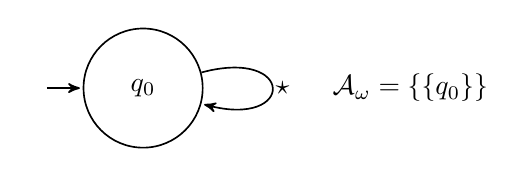
\begin{tikzpicture}[->,>=stealth',shorten >=1pt,auto,node distance=2.8cm,semithick,initial text={}]
  \tikzstyle{every state}=[minimum size=10ex]
  \tikzstyle{register}=	[circle,fill,draw,inner sep=0pt,minimum size=2pt]
	
  \node[state,initial] (q0) {$q_0$}; 
  \node[right=10ex of q0] {$\acc_\omega = \{ \{q_0 \}\}$ };

  \path (q0) edge [loop right]  node[inner sep=1pt] (star) {$\star$} (q0);
\end{tikzpicture}

\end{center}
\caption{Automaton $\autom_\omega$ for $\names^\omega$.}
\label{fig:nomega-automaton}
\end{figure}

\begin{figure}[t]
\begin{center}
 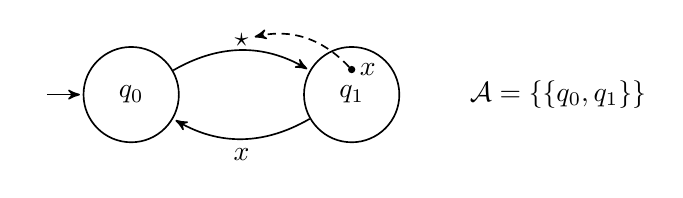
\begin{tikzpicture}[->,>=stealth',shorten >=1pt,auto,node distance=2.8cm,semithick,initial text={}]
  \tikzstyle{every state}=[minimum size=8ex]
  \tikzstyle{register}=	[circle,fill,draw,inner sep=0pt,minimum size=2pt]
	
  \node[state,initial] (q0) {$q_0$}; 
  \node[state,right of=q0] (q1) {};  
  \node (lab1) at (q1) {$q_1$};
  \node[register,label={[xshift=-2pt]right:$x$}] (reg) [above=1pt of lab1] {};
  \node [right=5ex of q1] {$\acc = \{ \{ q_0,q_1 \} \}$};


  \path (q0) edge [bend left]  node[inner sep=1pt] (star) {$\star$} (q1);
  \path (q1) edge [bend left] node {$x$} (q0);
  \path (reg) edge[densely dashed,bend right] (star);
\end{tikzpicture}
\end{center}
\caption{\label{fig:upwords} Automaton for the language of \cref{exa:session}.}
\end{figure}

\tbox{Sezione 4?}
{
Given a sequence $P$ of transitions in $A$, we write $(q_1,\rho_1) \TrP{v}{P} (q_2,\rho_2)$ whenever $(q_1,\rho_1) \Tr{v} (q_2,\rho_2)$ and such path is induced by $P$.
}
%
An \emph{ultimately periodic} word is a word of the form $uv^\omega$, with $u,v \in \names^\star$.  It is well known that each non-empty $\omega$-regular language $\Lang$ contains at least one such word \cite{CalbrixNP93}. In fact, given any $\alpha \in \Lang$, the run $r^\alpha$ in a Muller automaton for $\Lang$ goes through two states $r^\alpha_i,r^\alpha_j$, $i<j$, such that $\{r^\alpha_i,r^\alpha_{i+1},\dots,r^\alpha_j\}$ is an accepting set and $r^\alpha_i = r^\alpha_j$. Intuitively: a loop through an accepting set of states is eventually encountered while recognizing $\alpha$. Call $u$ the word recognized until $r^\alpha_i$, and $v$ the word recognized along the loop, then we clearly have $uv^\omega \in \Lang$.

In this section we prove an analogous result for nominal $\omega$-regular languages. This again involves finding a loop through accepting states and iterating it, but such loop must be in the configuration graph, i.e.\ it must be a path starting and ending with the same state \emph{and} register assignment.
%The following example gives evidence of this point.
%To illustrate this point:
%
%, unfortunately, it may not be possible to recognize the same word in subsequent traversals of the loop. The figure... illustrates this point:
%To illustrate this point, consider the \hdma{} in figure...
%
%\begin{example}
%Consider the automaton $A$ in \cref{fig:upwords}: it has a loop from $q_0$ to itself. Unlike ordinary Muller automata, the same symbol cannot be consumed by two subsequent iterations of the loop, because of the freshness requirement. However, the same symbol can be consumed after (at least) \emph{two} iterations, as illustrated by the following path in the configuration graph of $A$:
%\[
%	(q_0,x \mapsto c) \tr{a} (q_0,x \mapsto a) \tr{b} (q_0,x \mapsto b) \tr{a} (q_0,x \mapsto a) \dots
%\]
%\end{example}
%
%
%\tbox{Mettere nell'appendice?}
%{
%\begin{lemma}
%\label{lem:tr-names}
%For all edges in the configuration graph $(p_1,\rho_1) \tr{a} (p_2,\rho_2)$ we have $\Im(\rho_2) \subseteq \Im(\rho_1) \cup \{ a \}$.
%\end{lemma}
%}
%
Most of this section will be spent in showing that, given a loop in a \hdma, we can always find a path as required, induced by consecutive traversals of the loop.

From now on we fix a loop (the specific \hdma{} is unrelevant)
\[
	L \;:=\; p_0 \htr{l_0}{\sigma_0} p_1 \htr{l_1}{\sigma_1} \dots \htr{l_{n-1}}{\sigma_{n-1}} p_0
\]
We write $\ul{i}$ for $i \mod n$. Let $\widehat{\sigma}_i \colon \weight{p_\ul{i+1}} \pto \weight{p_i}$ be the partial maps telling the history of old registers and ignoring the new ones, formally
\[
	\widehat{\sigma}_i := \sigma_i \setminus \{ (x,y) \in \sigma_i \mid y = \star \} 
	\qquad (i=0,\dots,n-1)
\]
and let $\widehat{\sigma} \colon \weight{p_0} \pto \weight{p_0}$ be their composition $\widehat{\sigma}_0 \circ \widehat{\sigma}_1 \dots \circ \widehat{\sigma}_{n-1}$. We define the set $I$ as the greatest subset of $\dom(\widehat{\sigma})$ such that $ \widehat{\sigma}(I) = I$,
i.e.\ $I$ are the registers of $p_0$ that ``survive'' along $L$. We denote by $T$ all the other registers, namely $T := \weight{p_0} \setminus I$. These are registers whose content is eventually discarded (not necessarily within a single loop traversal), as the following lemma states.
%
%
\begin{lemma}
\label{lem:rho-forget}
Given any $x \in T$, let $\{x_j\}_{j \in J_x}$ be the smallest sequence that satisfies the following conditions:
$
	x_0 = x
$
and
$
	x_{j+1} = \sigma_{\ul{j}}^{-1}(x_j),
$
where $j+1 \in J_x$ only if $\sigma_{\ul{j}}^{-1}(x_i)$ is defined. Then $J_x$ has finite cardinality.
\end{lemma}
%
Now, consider any assignment $\rrho_0 \colon \weight{p_0} \to \names$. We give some lemmata about paths that start from $(p_0,\rrho_0)$ and are induced by consecutive traversals of $L$. The first one says that the assignment for $I$ given by $\rrho_0$ is always recovered after a fixed number of traversals of $L$, regardless of which symbols are consumed.
%
\begin{lemma} 
\label{lem:idI}
There is $\id \geq 1$ such that,
%there is $\id \geq 1$ such that, 
for all $v_0,\dots,v_{\id-1}$ satisfying
\[
	(p_0,\rrho_0) \TrP{v_0}{L} (p_0,\rrho_1) \TrP{v_1}{L} \dots \TrP{v_{\id-1}}{L} (p_0,\rrho_\id)
\]
we have $\restr{ \rrho_\id }{I} = \restr{ \rrho_0 }{I}$.
\end{lemma}
%
The second one says that, after a minimum number of traversals of $L$, a configuration can be reached where the initial values of $T$, namely those assigned by $\rrho_0$, cannot be found in any of the registers.
%
\begin{lemma}
There is $\forg \geq 1$ such that, for all $\gamma \geq \forg$ ,there are $v_0,\dots,v_{\gamma-1}$ satisfying
\[
	(p_0,\rrho_0) \TrP{v_0}{L} (p_0,\rrho_1) \TrP{v_1}{L} \dots \TrP{v_{\gamma-1}}{L} (p_0,\rrho_\gamma)
	\qquad 
	\Im(\rrho_\gamma) \cap \rrho_0(T) = \varnothing \enspace .
\]
%(Fix: $\rrho_0(\weight{p_0}) \cap \rrho_\gamma(T) = \varnothing$?)
\label{lem:forgetT}
%there is $\ass$ such that, 
\end{lemma}
%
%\vspace{-5ex}
%
Finally, we give the dual of the previous lemma: if we start from a configuration where registers are not assigned values in $\rrho_0(T)$, then these values can be assigned back to $T$ in a fixed number of traversals of $L$, regardless of the initial assignment.

\begin{lemma}
There is $\ass \geq 1$ such that,
for any $\trho_0 \colon \weight{p_0} \to \names$ with $\Im(\trho_0) \cap \rrho_0(T) = \varnothing$, there are $v_0,\dots,v_{\ass-1}$ satisfying
\[
	(p_0,\trho_0) \TrP{v_0}{L} (p_0,\trho_1) \TrP{v_1}{L} \dots \TrP{v_{\ass-1}}{L} (p_0,\trho_\ass)	
	\qquad
	\restr{\trho_\ass}{T} = \restr{\rrho_0}{T} \enspace .
\]
%and $\restr{\trho_\ass}{T} = \restr{\rrho_0}{T}$.
\label{lem:initT}
\end{lemma}
%
\vspace{-4ex}
%
Finally, we combine the above lemmata. We construct a path where: (1) the values assigned to $T$ are forgotten and then recovered (2) the values assigned to $I$ are swapped, but the initial assignment is periodically regained. Therefore, the length of such path should allow (1) and (2) to ``synchronize'', so that the final assignment is again $\rrho_0$.

\begin{theorem}
\label{thm:loop}


There are $v_0,\dots,v_n$ such that
\[
	(p_0, \rrho_0) \TrP{v_0}{L} (p_0, \rrho_1) \TrP{v_1}{L} \cdots \TrP{v_n}{L} (p_0,\rrho_0) \enspace .
\]
\end{theorem}

\begin{proof}
We can take any path of the form
\[
	(p_0,\rrho_0) \TrP{v_0}{L} (p_0,\rrho_1) \TrP{v_1}{L} \cdots \TrP{v_{\gamma-1}}{L} (p_0,\rrho_\gamma) \TrP{v_{\gamma}}{L} \cdots \TrP{v_{\gamma + \ass - 1}}{L} (p_0,\rrho_{\gamma + 
	 \ass})
\]
where the part from $(p_0,\rrho_0)$ to $(p_0,\rrho_\gamma)$ is given by \cref{lem:forgetT} and the remaining subpath is given by \cref{lem:initT}, with $\trho_0 = \rrho_\gamma$. The only constraint about $\gamma$ is that there should be a positive integer $\lambda$ such that $\gamma + \ass = \lambda \id$, where $\id$ is given by \cref{lem:idI}. The claim follows from $\restr{\rrho_{\gamma + \ass}}{T} = \restr{\rrho_0}{T}$ and 
$\restr{\rrho_{\gamma + \ass}}{I} = \restr{\rrho_0}{I}$ which, together with $I \cup T = \weight{p_0}$, imply $\rrho_{\gamma + \ass} = \rrho_0$.
\qed
\end{proof}
%

\begin{figure}[t]
\begin{center}
 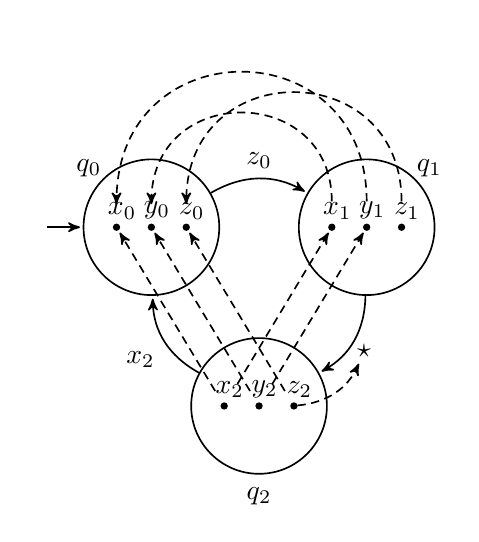
\begin{tikzpicture}[->,>=stealth',shorten >=1pt,auto,node distance=2.8cm,semithick,initial text={}]
  \tikzstyle{every state}=[minimum size=10ex]
  \tikzstyle{register}=	[circle,fill,draw,inner sep=0pt,minimum size=2pt]
	
  %\node[state,right of=q0] (q1) {};
  %\node[state,right of=q1] (q2) {};

  %\node (lab0) at (q0) {$q_0$};
  %\node (lab1) at (q1) {$q_1$};
  %\node (lab2) at (q2) {$q_2$};

  \node[register,label={[shift={(2pt,-2pt)}]above:$x_0$}] (reg00) {};
  \node[register,label={[shift={(2pt,-2pt)}]above:$y_0$}] (reg01) [right=10pt of reg00] {};
  \node[register,label={[shift={(2pt,-2pt)}]above:$z_0$}] (reg02) [right=10pt of reg01] {};

  \node[register,label={[shift={(2pt,-2pt)}]above:$x_1$}] (reg10) [right=50pt of reg02] {};
  \node[register,label={[shift={(2pt,-2pt)}]above:$y_1$}] (reg11) [right=10pt of reg10] {};
  \node[register,label={[shift={(2pt,-2pt)}]above:$z_1$}] (reg12) [right=10pt of reg11] {};

  \node[register,label={[shift={(2pt,-2pt)}]above:$y_2$}] (reg21) at ($(reg02)!0.5!(reg10)$) [yshift=-15ex] {};
%[right=10pt of reg20] {};

  \node[register,label={[shift={(2pt,-2pt)}]above:$x_2$}] (reg20) [left=10pt of reg21] {};
  \node[register,label={[shift={(2pt,-2pt)}]above:$z_2$}] (reg22) [right=10pt of reg21] {};



  \node[state,initial,fit={(reg00) (reg01) (reg02)},inner sep=2ex] (q0) {};
  \node[above left=-1ex of q0] (lab0) {$q_0$};
%,label={[anchor=north west]above:$q_0$}] (q0) {$q_0$}; 
  \node[state,fit={(reg10) (reg11) (reg12)},inner sep=2ex] (q1) {};
  \node[above right=-1ex of q1] (lab1) {$q_1$}; 
  \node[state,fit={(reg20) (reg21) (reg22)},inner sep=2ex] (q2) {};
  \node[below=1pt of q2] (lab2) {$q_2$}; 
%  \node [left=10ex of reg,inner sep=0pt] (c) {$c$};
  %\node[state,right of=q0] (q1) {$q_1$};  

  \path (q0) edge [bend left] node {$z_0$} (q1);
  \path (q1) edge [bend left]  node[inner sep=1pt] (star) {$\star$} (q2);
  \path (q2) edge [bend left] node {$x_2$} (q0);
	
  \path (reg10) edge[densely dashed,out=90,in=90,looseness=2,shorten >=7pt,shorten <=8pt] (reg01);
  \path (reg11) edge[densely dashed,out=90,in=90,looseness=2,shorten >=7pt,shorten <=8pt] (reg00);
  \path (reg12) edge[densely dashed,out=90,in=90,looseness=2,shorten >=7pt,shorten <=8pt] (reg02);

  \path (reg20) edge[densely dashed,shorten <=8pt] (reg10);
  \path (reg21) edge[densely dashed,shorten <=8pt] (reg11);
  \path (reg22) edge[bend right,densely dashed] (star);

  \path (reg20) edge[densely dashed,shorten <=5pt] (reg00);
  \path (reg21) edge[densely dashed,shorten <=5pt] (reg01);
  \path (reg22) edge[densely dashed,shorten <=5pt] (reg02);

%  \path (reg00) edge[dashed,bend right=50] (star);
 % \path (reg00) edge[dashed] (c);
%  \draw[dashed,bend left] (reg) -- (star);
%             edge [loop left]  node {a} (q0)
%        (q1) edge [bend left]  node {a} (q0)
%             edge [loop right] node {b} (q1);
\end{tikzpicture}

\end{center}
\caption{\label{fig:upwords-ex} An example automaton. Some transitions are not shown: they are all assumed to end up in a sink state without registers.}
\end{figure}

\begin{example} We justify the above construction on the automaton in \cref{fig:upwords-ex}, with initial assignment $\rho_0(x_0) = a$,$\rho_0(y_0) = b$ and $\rho_0(z_0) = c$. We omit the accepting set, as it is not relevant. Consider the loop $L$ formed by all the depicted transitions.
We have $I = \{x_0,y_0\}$ and $T = \{z_0\}$. Consider the path
\[
	(q_0,[\subs{a}{x_0},\subs{b}{y_0},\subs{c}{z_0}]) \tr{c} (q_1,[\subs{b}{x_1},\subs{a}{y_1},\subs{c}{z_1}]) \tr{d} (q_2,[\subs{b}{x_2},\subs{a}{y_2},\subs{d}{z_2}]) \tr{b} (q_0,[\subs{b}{x_0},\subs{a}{y_0},\subs{d}{z_0}])
\]
where $d \neq a,b,c$. Notice that the values of $x_0$ and $y_0$ get swapped according to the permutation $(a \; b)$, and $d$ is assigned to $z_0$. Our aim is to recover $\rho_0$ again. According to \cref{lem:idI}, $x_0$ and $y_0$ get their assignment back in $\theta = 2$ traversals of $L$ (in fact $(a\; b)^2 = (a\; b)$). As for $z_0$, its assignment is established in the second transition, but $c$ should not have been assigned to any register of $q_1$ in order for it to be consumed during this transition. This is where \cref{lem:forgetT} comes into play: it says that in at least $\epsilon = 1$ traversals of $L$ the name $c$ is discarded. This is exactly what happens in the path shown above. Then we can assign $c$ to $z_0$ in another $\zeta = 1$ traversal of $L$, according to \cref{lem:initT}. Since $\epsilon + \zeta  = \theta = 2$, traversing $L$ twice is enough. For instance, we can take the path spelling $cdbdca$.
\end{example}


Finally we have the main theorem.
%
\begin{theorem}
Every non-empty $\omega$-regular nominal language $\Lang$ has an ultimately periodic fragment.
\end{theorem}
\begin{proof}
Let $\autom$ be the automaton for $\Lang$. Take any $\alpha \in \Lang$ and let $I = \Inf(r^\alpha)$ (recall $r^\alpha$ is the run for $\alpha$ in $\autom$), so $I \in \acc$. A path spelling $\alpha$ in the configuration graph of $A$ must \todo{Spiegare meglio perchè ``must''?} begin with
\[
	(q_0,\rho_0) \Tr{u} (q_1,\rho_1) \TrP{v}{P} (q_1,\rho_2)
\]
where $q_1 \in I$ and $(q_1,\rho_1) \TrP{v}{P} (q_2,\rho_2)$ is such that $P$ goes through all the states in $I$. Since $P$ is a loop, we can replace its induced path with a new one given by \cref{thm:loop} 
\[
	(q_0,\rho_0) \Tr{u} (q_1,\rho_1) \TrP{v_0}{P} \cdots \TrP{v_n}{P} (q_1,\rho_1) \enspace .
\]
This subpath can be traversed any number of times, so we have $u(v_0\dots v_n)^\omega \in \Lang$.
\qed
\end{proof}


%\section{Nominal regularity of looping fragments}\label{sec:regularity-of-loop}%!TEX root=ndma.tex
\newcommand{\eq}[1]{=_{#1}}

Given two \hdmas{} $\autom_i = (Q_i,\weight{-}_i,q_0^i,\rho_0^i,\trarrow_i,\acc_i)$, $i=1,2$, we now define their \emph{synchronized product} $\autom_1 \syncp \autom_2$. We assume $\weight{q_1}_1 \cap \weight{q_2}_2 = \varnothing$, for all $q_i \in Q_i$.\todo{Dare lemma in cui si dice che posso sempre rinominare i registri?} Some notation: given two disjoint sets of names $S_1,S_2 \subseteq \names$,we write $Eq(S_1,S_2)$ for the set of all equivalence relations $R \subseteq (S_1 \cup S_2) \times (S_1 \cup S_2)$ induced by equations of the form $x_1 \eq{R} x_2$, for $x_i \in S_i$. 

\begin{definition}[Synchronized product of \hdmas]
\label{def:syncp}
 $\autom_1 \syncp \autom_2$ is an automaton $(Q,\weight{-},q_0,\rho_0,\trarrow_i,\acc)$ defined as follows
\begin{itemize}
	\item $Q := \bigcup_{q_1 \in Q_1,q_2 \in Q_2} \{(q_1,q_2)\} \times Eq(\weight{q_1}_1,\weight{q_2}_2)$;
	%
	\item $\weight{(q_1,q_2,R)} := (\weight{q_1}_1 \cup \weight{q_2}_2)_{/R}$, for $(q_1,q_2,R) \in Q$;
	%
	\item $q_0 := (q_0^1,q_0^2,R_0)$, where $R_0$ is given by
	\[
		\inferrule
		{ \rho_0^1(x_1) = \rho_0^2(x_2) \\ x_1 \in \weight{q_0^1},x_2 \in \weight{q_0^2}}
		{ x_1 \eq{R_0} x_2 }
	\]
	\item $\rho_0([x]_{R_0}) = \rho_0^i (x)$ whenever $x \in \weight{q_0^i}_i$, $i \in \{1,2\}$; 
	%(well-defined by definition of $R_0$);
	%
	\item $(q_1,q_2,R) \htr{l}{\sigma} (q_1',q_2',R')$ if and only if there are $q_i \htrind{l_i}{\sigma_i}{i} q_i'$, $i=1,2$, such that $\sigma([x]_{R'}) = [\sigma_i(x)]_R$, for all $x \in \weight{q_i'}$ with $\sigma_i^{-1}(x) \neq \star$, 
	%for $i \in \{1,2\}$ $i=1,2$ 
	%$q_2 \htrind{l_2}{\sigma_2}{2} q_2'$, 
	and one of the following holds: 
	\begin{itemize}
		%	
		\item if $l_1,l_2 \in \names$ then $l_1 =_R l_2$, $l = [l_1]_R$, and $R'$ is the smallest equivalence relation generated by
		\[
			\inferrule*[left=Eq]
			{ x_1 \eq{R} x_2 \\ x_1 \in \Im(\sigma_1),x_2 \in \Im(\sigma_2)}
			{ \sigma_1^{-1}(x_1) \eq{R'} \sigma_2^{-1}(x_2) }
		\]
		%
		\item if $l_1 \in \names$ and $l_2 = \star $ then $l = [l_1]_R$, $[l_1]_R = \{l_1\}$ and $R'$ is generated by \textsc{Eq} and
		\[
			\inferrule
			{ l_1 \in \Im(\sigma_1) }
			{ \sigma_1^{-1}(l_1) \eq{R'} \sigma_2^{-1}(\star) }
		\]
		and $\sigma([\sigma_2^{-1}(\star)]_{R'}) = [l_1]_R$.
		\item if $l_1,l_2 = \star$ then $l=\star$ and $R'$ is generated by \textsc{Eq} and
		\[
			\sigma_1^{-1}(\star) \eq{R'} \sigma_2^{-1}(\star)
		\]
		and $\sigma([\sigma_1^{-1}(\star)]_{R'}) = \star$.
	\end{itemize}
	%and $\sigma([x]_{R'}) = [\sigma_i(x)]_R$ whenever $x \in \weight{q_i'}$, for $i \in \{1,2\}$.
%		\[
%			\sigma([x]_{R'}) = 
%			\begin{cases}
%				[\sigma_1(x)]_R & x \in \weight{q_1'} \\
%				[\sigma_2(x)]_R & x \in \weight{q_2'}
%			\end{cases}
%		\]
\end{itemize}
\end{definition}

\begin{proposition}
Let $((q_1,q_2,R),\rho) \tr{a} ((q_1',q_2',R'),\rho')$ be an edge in the configuration graph of $\autom_1 \syncp \autom_2$, and let $\rho_i = \lambda x \in \weight{q_i}.\rho([x]_R)$, for $i=1,2$. Then $(q_i,\rho_i) \trind{a}{i} (q_i',\rho_i')$ is and edge in the configuration graph of $\autom_i$ with $\rho'_i = \lambda x \in \weight{q_i}.\rho'([x]_{R'})$.
%, for $i=1,2$.
%and $(q_2,\rho_2) \trind{a}{2} (q_2',\rho_2')$ are edges in the configuration graphs of $\autom_1$ and $\autom_2$, respectively, with $\rho'_i = \lambda x \in \weight{q_i}.\rho'([x]_{R'})$.
\end{proposition}
\begin{proof}
We proceed by cases on the transition $((q_1,q_2,R),\rho) \htr{l}{\sigma} ((q_1',q_2',R'),\rho')$ in $\autom_1 \syncp \autom_2$ that induces $((q_1,q_2,R),\rho) \tr{a} ((q_1',q_2',R'),\rho')$:
\begin{description}
	\item[Case $l \in \names$:] Then there are two transitions $q_i \htrind{l_i}{\sigma_i}{i} q_i'$, $i=1,2$, according to \cref{def:syncp}.
	% and $q_2 \htrind{l_2}{\sigma_2}{2} q_2'$ according to \cref{def:syncp}. 
	We have two cases:
	\begin{itemize}
	\item $l_1,l_2 \in \names$.
	Since $l_1 \eq{R} l_2$, we have $\rho_i(l_i) = \rho([l_i]_R) = \rho([l]_R) = a$, so these transitions induce two edges $(q_i,\rho_i) \trind{a}{i} (q_i',\rho_i')$.
	% and $(q_2,\rho_2) \trind{a}{2} (q_2',\rho_2')$.
	Given $x \in \weight{q_i'}$, the following chain of equations, all expanding the definition of the involved function, proves the last part of the statement
	\begin{align*}
		\rho'_i(x) &= \rho_i (\sigma_i (x) ) \\
		&= \rho([\sigma_i(x)]_R) \\
		%&& \text{(by definition of $\rho_i$)}\\
		&= \rho(\sigma([x]_{R'})) \\
		%&& \text{(by definition of $\sigma$)}\\
		&= \rho'([x]_{R'}) 
		%&& \text{(by definition of $\rho'$)}
	\end{align*}
	
	\item if $l_1 \in \names,l_2 = \star$ then $\rho_1(l_1) = \rho([l_1]_R) = a$ and $a \notin \Im(\rho_2)$. In fact, %$a \in \Im(\rho_2)$ only 
	if there was $l_2 \in \weight{q_2}$ such that $\rho_2(l_2) = a$, then $\rho([l_2]_R) = a = \rho([l_1]_R)$, by definition of $\rho$, which implies $[l_1]_R = [l_2]_R$, by injectivity of $\rho$, i.e. $\{l_1,l_2\} \in [l_1]_R$, against the hypothesis $[l_1]_R = \{l_1\}$. So we have $(q_i,\rho_i) \trind{a}{i} (q_i',\rho_i')$, $i=1,2$, and the same equations as the previous case hold; we just have to check the value of $\rho_2'$ on $x = \sigma_2^{-1}(\star)$:
	\begin{align*}
		\rho'_2(x) &= (\rho_2 \circ \sigma_2)\sub{a}{\sigma_2^{-1}(\star)}(x) \\
		&= a \\
		&= \rho([l_1]_R) \\
		&= (\rho \circ \sigma)([x]_{R'}) \\
		& = \rho'([x]_{R'})
	\end{align*}	
	All the equations just apply the definitions of the involved functions.
	%so $\rho([l_1]_R) = \rho([l_2]_R)$, by injectivity of $\rho$.
	%, but this means $, because $[l_1]_R = \{l_1\}$
	\end{itemize}

	\item[Case $l = \star$:] 
	Then we have $q_i \htrind{\star}{\sigma_i}{i} q_i'$, and for $i=1,2$% and $x = \sigma_i^{-1}(\star)$
	\begin{align*}
		\rho'_i(\sigma_i^{-1}(\star)) &= (\rho_i \circ \sigma_i)\sub{a}{\sigma_i^{-1}(\star)}(\sigma_i^{-1}(\star)) \\
		&= a \\
		&= (\rho \circ \sigma) \sub{a}{\sigma^{-1}(\star)}(\sigma^{-1}(\star)) \\
		&= (\rho \circ \sigma) \sub{a}{[\sigma_1^{-1}(\star)]_{R'}}([\sigma_1^{-1}(\star)]_{R'}) \\
		%&& \text{(by $[\sigma_1^{-1}(\star)]_{R'} = [\sigma_i(\star)^{-1}]_{R'}$)} \\
		& = (\rho \circ \sigma) \sub{a}{[\sigma_i^{-1}(\star)]_{R'}}([\sigma_i^{-1}(\star)]_{R'}) && \text{(definition of $R'$)} \\
		&= \rho'([\sigma_i(\star)^{-1}]_{R'})
	\end{align*}
	
	%Then there are $q_i \htrind{l_i}{\sigma_i}{i} q_i'$, $i=1,2$. We have two cases:
%	\begin{itemize}
%		\item 
%	\end{itemize}
\end{description} 
\end{proof}

\begin{corollary}
Given a path $((q_0^1,q_0^2,R_0),\rho_0) \tr{a_0} \dots \tr{a_{n-1}} ((q_n^1,q_n^2,R_n),\rho_n)$ in the configuration graph of $\autom_1 \syncp \autom_2$, there is a path $(q_0^i,\rho_0^i) \tr{a_0} \dots \tr{a_{n-1}} (q_n^i,\rho_n^i)$ in the configuration graph of $\autom_i$ with $\rho_n^i = \lambda x \in \weight{q_n^i}.\rho_n([x]_{R_n})$, for $i=1,2$.
\end{corollary}

\begin{proposition}
$\syncp$ is associative.
\end{proposition}


%\section{Decidability}\label{sec:decidability}%!TEX root=ndma.tex

%\todo{Quick introduction to \cite{CV12}}
% not really needed
\begin{theorem}
It is decidable whether $\Lang$ is the empty language.
\label{thm:emptiness}
\end{theorem}

\begin{theorem}
It is decidable whether $\Lang_1 = \Lang_2$.
\end{theorem}

\begin{proof}
Consider the language $\Lang = (\Lang_1 \cup \Lang_2) \setminus (\Lang_1 \cap \Lang_2 )$. This is $\omega$-regular nominal, thanks to \cref{thm:bool-closure}. Then we just have to check the emptiness of $\Lang$, which is decidable by \cref{thm:emptiness}.
\end{proof}

\section{Conclusions}\label{sec:conclusions}
This work is an attempt to provide a simple definition that merges the theories of nominal automata and $\omega$-regular languages, retaining effective closure under boolean operations, and determinacy by ultimately periodic words. We sketch some possible future directions. It is well known that nominal set correspond to sheaves over the \emph{atomic topology}, which form a subcategory of a presheaf category indexed by finite sets \cite{fabio,staton}. By changing the index category, one may express more complex relations among symbols in the alphabet, such as, graph-based network topologies \cite{matteo}. Extending nDMA to work in such a richer setting seems relevant. For example, using graphs, one could predicate on arbitrary relations between symbols, and require that infinitely often, one passes by a symbol which is related in a certain way to a number of its predecessors. Furthermore, recall that automata correspond to logic formulae. Nominal Muller automata could be put in correspondence with logic formulae with binders. However, there may be different logical interpretations of automata, where causality or dependence between events are made explicit. Finally, extending the two-sorted setting of \cite{CV12} to hDMAs would enhance the defined framework with canonical representatives of automata, up-to language equivalence.

%!TEX root=ndma.tex
\begin{itemize}
	\item LTL with the Freeze Quantifier and Register Automata (Demri Lazic): 
\end{itemize}

\paragraph{Acknowledgements.} The authors would like to thank Nikos Tzevelekos, Emilio Tuosto and Gianluca Mezzetti for several fruitful discussions related to nominal automata.

\bibliographystyle{splncs}
\bibliography{biblio_matteo,biblio_vincenzo,thesis_biblio}


\appendix
\section{Proofs}
%!TEX root=ndma.tex

\begin{lemma}
\label{lem:xI}
Given $x \in \dom(\widehat{\sigma})$, suppose there is a positive integer $k$ such that $x = \widehat{\sigma}^k (x)$. Then $x \in I$.
\end{lemma}
\begin{proof}
Suppose $x \notin I$. $I = \widehat{\sigma}(I)$ implies $I = \widehat{\sigma}^k(I)$, so $I \cup \{x\} = \widehat{\sigma}^k(I \cup \{x\})$, but this is against the assumption that $I$ is the largest set satisfying $I = \widehat{\sigma}(I)$.
\qed
\end{proof}


\begin{proof}[of \cref{lem:rho-forget}]
Suppose $|J_x| \geq n$, otherwise the statement is trivially true. Observe that this sequence is such that $x_{kn} \neq x_{k'n}$, for all $k,k' \geq 0$ such that $k \neq k'$. In fact, suppose there are $x_{kn} = x_{k'n}$, with $k < k'$. Then we would have $x_{kn-1} = x_{k'n-1}$, because $\sigma_{n}$ is injective. In general, $x_{kn-l} = x_{k'n-l}$, for $0 \leq l \leq kn$, therefore $x = x_0 = x_{(k'-k)n}$. This means that $\widehat{\sigma}^{(k'-k)}(x) = x$ which, by \cref{lem:xI}, implies $x \in I$, against the hypothesis $x \in T$.

Now, suppose that $J_x = \mathbb{N}$. Then we would have an infinite subsequence $\{x_{jn}\}_{j \in J_x}$ of pairwise distinct names that belong to $\weight{p_0}$, but $\weight{p_0}$ is finite, a contradiction.
\qed
\end{proof}


\begin{proof}[of \cref{lem:IT}]\hfill
\begin{enumerate}[(i)]


\item Let $\pi \colon I \to I$ be the function $\restr{\widehat{\sigma}}{I}$ with its codomain restricted to $I$. Then $\pi$ is an element of the symmetric group on $I$, so it has an order $\id$, that is a positive integer such that $\pi^\id = id_I$\todosm{Dovrebbe funzionare sempre con $\id = |I|!$, cioè con l'ordine del gruppo}. Hence $\restr{ \rrho_\id }{ I } =\restr{ \rrho_0 }{I} \circ \pi^\id = \restr{ \rrho_0 }{I}$.


\item
Let $\mathcal{J}$ be
\[
	\mathcal{J} := \max \{ |J_x|\mid x \in T \} + 1 .
\]
This gives the number of transitions it takes to forget all the names stored in $T$. Let $\forg$ be $\lceil \frac{\mathcal{J}}{n} \rceil$. For any $\gamma \geq \forg$, we can choose $v_1,\dots,v_\gamma$ as any $\gamma$-tuple of words that are recognized by the loop and such that, whenever $l_j = \star$, then $(v_i)_j$ is different from $\Im(\rrho_0)$ and all the previous symbols in $v_1,\dots,v_i$, for all $i=1,\dots,\gamma$ and $j=1,\dots,n$. Let us verify $\Im(\rrho_\gamma) \cap \rrho_0(T) = \varnothing$ separately on $I$ and $T$ (recall $I \cup T = \weight{p_0})$: we have $\rrho_\gamma(T) \cap \rrho_0(T) = \varnothing$, because all the names assigned to $T$ have been replaced by fresh ones; and we have $\rrho_\gamma(I) = \rrho_0(I)$, so $\rrho_\gamma(I) \cap \rrho_0(T) = \varnothing$.
\end{enumerate}
\qed
\end{proof}


\begin{proof}[of \cref{lem:initT}]
For each name $x \in T$ define a tuple $(x,i,j)$ where $i$ is the index of the transition where $x$ is allocated and $j$ is the number of loop traversals needed to allocate it, i.e.\ $j$ is the smallest integer such that there are $x_{jn},\dots,x_1$ defined as follows
\[
	x_{jn} = x \qquad \sigma_\ul{k+1}(x_{k+1}) = x_k \qquad \sigma_i(x_1) = \star
\]
Let $X$ be the set of such tuples and let $\ass := \max \{ j \mid (x,i,j) \in X \}$. Then we can construct $v_1,\dots,v_\ass$ as follows
\[
	(v_k)_i :=
	\begin{cases}
		\text{$y$ fresh} & l_i = \star \land i \notin \pi_2(X) \\
		\rrho_0(x) & (x,i,\ass - k + 1)\footnotemark \in X
		 \\
		%\trho_0(l_0) & l_0 \neq \star \\
		\trho_{k-1}(l_i) & l_i \neq \star
	\end{cases}
\]

where by $y$ fresh we mean different from elements of $\Im(\trho_0) \cup \Im(\rrho_0)$ and previous symbols in $v_1,\dots,v_{k}$.

The second case in the definition of $(v_k)_i$ is justified as follows. Suppose $\trho_{k,i}$ is the register assignment for the transition $(p_i,\trho_{k,i}) \tr{(v_k)_i} \dots$, then we have to show $(v_k)_i = \rrho_0(x) \notin \Im(\trho_{k,i})$. Suppose, by contradiction, that $\rrho_0(x) \in \Im(\trho_{k,i})$, then by \cref{lem:tr-names} we have $\rrho_0(x) \in \Im(\trho_0) \cup F$, where $F$ are all the fresh names allocated so far. But $F \cap \Im(\rrho_0) = \varnothing$, by construction, so $\rrho_0(x) \in \Im(\trho_0)$, which implies $\rrho_0(T) \cap \Im(\trho_0) \neq \varnothing$, due to $x \in T$, against our hypothesis.

It is easy to see that $\trho_\ass$ satisfies the statement by construction.
\qed
\end{proof}


\end{document}
